\documentclass[11pt]{article}
\usepackage{amsmath, amssymb, physics, mathtools, bm}
\usepackage{tikz, pgfplots}
\pgfplotsset{compat=1.18}
\usepackage[margin=2.3cm]{geometry}
\usepackage{siunitx, booktabs, hyperref}
\usepackage{braket}

\newcommand{\D}{\mathrm{D}}
\newcommand{\de}{\mathrm{d}}
\newcommand{\pd}[2]{\frac{\partial #1}{\partial #2}}
\newcommand{\pdd}[2]{\frac{\partial^{2} #1}{\partial #2^{2}}}
\newcommand{\Lap}{\nabla^{2}}

\title{B6 Condensed-Matter Physics --- Model Solutions, 2019}
\author{}
\date{}

\begin{document}
\maketitle

%======================================================================
\section*{Question 1 --- Reciprocal lattice and powder diffraction}

\subsection*{(a) Lattice and basis}

\textbf{Problem.} \emph{Define the terms lattice and basis as they have been used in this course.}

\textbf{Lattice:} an infinite set of points $\{\bm R = n_1\bm a_1 + n_2\bm a_2 + n_3\bm a_3 : n_i\in\mathbb Z\}$ such that the environment seen from every point is identical (a Bravais lattice).

\textbf{Basis:} the group of one or more atoms (with positions $\bm r_p$ relative to a lattice point) that is repeated on every lattice site to build the crystal.

\subsection*{(b) Reciprocal lattice}

\textbf{Problem.} \emph{Given primitive lattice vectors $\bm a_1, \bm a_2, \bm a_3$, define the reciprocal lattice and prove the standard primitive vectors generate every $\bm G$ satisfying $\exp(i\bm G\!\cdot\!\bm R)=1$.}

Define
\begin{equation}
\bm b_1 = 2\pi\,\frac{\bm a_2\times\bm a_3}{\bm a_1\cdot(\bm a_2\times\bm a_3)},\qquad
\bm b_2 = 2\pi\,\frac{\bm a_3\times\bm a_1}{\bm a_1\cdot(\bm a_2\times\bm a_3)},\qquad
\bm b_3 = 2\pi\,\frac{\bm a_1\times\bm a_2}{\bm a_1\cdot(\bm a_2\times\bm a_3)}.
\label{eq:bdef}
\end{equation}
Orthogonality identity:
\[
\bm b_i\cdot\bm a_j = 2\pi\,\delta_{ij}.
\]
Take $\bm G=m_1\bm b_1+m_2\bm b_2+m_3\bm b_3$ with $m_i\in\mathbb Z$ and $\bm R=n_1\bm a_1+n_2\bm a_2+n_3\bm a_3$:
\[
\bm G\cdot\bm R = \sum_{i,j} m_i n_j\,(\bm b_i \cdot \bm a_j).
\]
Apply orthogonality $\bm b_i\cdot\bm a_j=2\pi\delta_{ij}$:
\[
\bm G\cdot\bm R = 2\pi\sum_i m_i n_i.
\]
Sum of integers is integer:
\[
\bm G\cdot\bm R \in 2\pi\mathbb Z.
\]
Hence $e^{i\bm G\cdot\bm R}=1$: every integer combination of $\bm b_i$ is a reciprocal lattice vector.

Conversely let $\bm G=\sum_i x_i\bm b_i$ with real $x_i$ satisfy $e^{i\bm G\cdot\bm R}=1$ for every lattice $\bm R$. Take $\bm R=\bm a_j$:
\[
\bm G\cdot\bm a_j = \sum_i x_i\,(\bm b_i \cdot \bm a_j).
\]
Apply orthogonality:
\[
\bm G\cdot\bm a_j = 2\pi x_j.
\]
Impose $e^{i\bm G\cdot\bm a_j}=e^{2\pi i x_j}=1$:
\[
x_j\in\mathbb Z.
\]
\boxed{\;\text{Every } \bm G \text{ is an integer combination of } \bm b_1,\bm b_2,\bm b_3.\;}

\subsection*{(c) Periodic Fourier transform}

\textbf{Problem.} \emph{Show that $V_{\bm q}=\int\de^3\bm x\,e^{i\bm q\cdot\bm x}V(\bm x)$ vanishes unless $\bm q$ is a reciprocal lattice vector.}

Shift integration variable $\bm x\to\bm x+\bm R$ for any lattice $\bm R$:
\[
V_{\bm q} = \int\de^3\bm x\, e^{i\bm q\cdot(\bm x+\bm R)} V(\bm x+\bm R).
\]
Use periodicity $V(\bm x+\bm R)=V(\bm x)$:
\[
V_{\bm q} = e^{i\bm q\cdot\bm R}\int\de^3\bm x\, e^{i\bm q\cdot\bm x}V(\bm x).
\]
Identify the remaining integral as $V_{\bm q}$:
\[
V_{\bm q} = e^{i\bm q\cdot\bm R}V_{\bm q}.
\]
Rearrange:
\[
(1-e^{i\bm q\cdot\bm R})V_{\bm q}=0 \quad \forall\bm R.
\]
\[
\boxed{\;V_{\bm q}=0\quad\text{unless } e^{i\bm q\cdot\bm R}=1\ \forall\bm R,\ \text{i.e.\ } \bm q=\bm G.\;}
\]

\subsection*{(d) Structure factor}

\textbf{Problem.} \emph{From $V(\bm x)=\sum_j u_j(\bm x-\bm x_j)$ and $\Gamma\propto|\langle\bm k'|V|\bm k\rangle|^2$, derive $I(\bm G)\propto|S(\bm G)|^2$ with $S(\bm G)=\sum_p b_p(\bm G)e^{i\bm G\cdot\bm r_p}$. Specify $b_p(\bm G)$.}

Plane waves $|\bm k\rangle\propto e^{i\bm k\cdot\bm x}$. Matrix element:
\[
\langle\bm k'|V|\bm k\rangle \propto \int\de^3\bm x\, e^{-i(\bm k'-\bm k)\cdot\bm x}V(\bm x).
\]
Identify with the Fourier component $V_{-\bm G}$, $\bm G\equiv\bm k'-\bm k$:
\[
\langle\bm k'|V|\bm k\rangle \propto V_{-\bm G}.
\]
Insert $V(\bm x)=\sum_j u_j(\bm x-\bm x_j)$:
\[
V_{-\bm G} = \sum_j\int\de^3\bm x\, e^{-i\bm G\cdot\bm x}u_j(\bm x-\bm x_j).
\]
Change variable $\bm y=\bm x-\bm x_j$:
\[
V_{-\bm G} = \sum_j e^{-i\bm G\cdot\bm x_j}\int\de^3\bm y\, e^{-i\bm G\cdot\bm y}u_j(\bm y).
\]
Define atomic form factor $\tilde u_j(\bm G)\equiv\int\de^3\bm y\, e^{-i\bm G\cdot\bm y}u_j(\bm y)$:
\[
V_{-\bm G} = \sum_j e^{-i\bm G\cdot\bm x_j}\,\tilde u_j(\bm G).
\]
Split $\bm x_j=\bm R + \bm r_p$ (lattice vector + basis position):
\[
V_{-\bm G} = \sum_{\bm R} e^{-i\bm G\cdot\bm R}\sum_{p\in\text{u.c.}} e^{-i\bm G\cdot\bm r_p}\tilde u_p(\bm G).
\]
Lattice sum gives $N_{\text{cell}}$ when $\bm G$ is a reciprocal lattice vector, else $0$:
\[
V_{-\bm G} = N_{\text{cell}}\sum_{p\in\text{u.c.}} e^{-i\bm G\cdot\bm r_p}\tilde u_p(\bm G).
\]
Square and absorb constants into $I(\bm G)\propto|V_{-\bm G}|^2$:
\[
\boxed{\;I(\bm G)\propto |S(\bm G)|^2,\quad S(\bm G)=\sum_{p\in\text{u.c.}} b_p(\bm G)\, e^{i\bm G\cdot\bm r_p},\quad b_p(\bm G)=\int\de^3\bm y\, e^{-i\bm G\cdot\bm y}u_p(\bm y).\;}
\]
(The sum over $j$ runs over every atom in the system; the sum over $p$ runs over the single-cell basis.)

\subsection*{(e) Powder pattern of silicon}

\textbf{Problem.} \emph{Si is fcc with two atoms per unit cell at $(0,0,0)$ and $\tfrac14(1,1,1)a$. Find $|\bm G|$ for the two lowest-angle powder rings.}

Conventional cubic reciprocal vectors $\bm G=(2\pi/a)(h,k,l)$. Fcc Bravais factor restricts to $h,k,l$ all-even or all-odd.

Basis sum with $\bm r_1 = 0$, $\bm r_2 = (a/4)(1,1,1)$:
\[
S_{hkl} \propto 1 + e^{i\bm G \cdot \bm r_2} = 1 + e^{i\pi(h+k+l)/2}.
\]
Vanishes when $(h+k+l)/2$ is odd:
\[
S=0\ \text{if}\ h+k+l\equiv 2\pmod 4.
\]
Test allowed $hkl$ in increasing $h^2+k^2+l^2$:
\[
(111):\ h^2+k^2+l^2=3,\quad h+k+l=3\ \text{(odd)} \Rightarrow \text{allowed}.
\]
\[
(200):\ =4,\quad h+k+l=2 \Rightarrow \text{forbidden}.
\]
\[
(220):\ =8,\quad h+k+l=4 \Rightarrow \text{allowed}.
\]
Magnitudes:
\[
|\bm G_{111}| = \frac{2\pi}{a}\sqrt{1^2+1^2+1^2}.
\]
Simplify:
\[
|\bm G_{111}| = \frac{2\pi\sqrt 3}{a}.
\]
For $(220)$:
\[
|\bm G_{220}| = \frac{2\pi}{a}\sqrt{2^2+2^2+0^2} = \frac{2\pi\sqrt 8}{a}.
\]
Simplify $\sqrt 8 = 2\sqrt 2$:
\[
|\bm G_{220}| = \frac{4\pi\sqrt 2}{a}.
\]
Plug in $a=\SI{5.43}{\angstrom}$:
\[
|\bm G_{111}| = \frac{2\pi\times 1.732}{5.43}\,\si{\angstrom^{-1}} \approx \SI{2.00}{\angstrom^{-1}}.
\]
\[
|\bm G_{220}| = \frac{2\pi\times 2.828}{5.43}\,\si{\angstrom^{-1}} \approx \SI{3.27}{\angstrom^{-1}}.
\]
\[
\boxed{\;|\bm G_{111}|=\frac{2\pi\sqrt 3}{a}\approx\SI{2.00}{\angstrom^{-1}},\qquad |\bm G_{220}|=\frac{4\pi\sqrt 2}{a}\approx\SI{3.27}{\angstrom^{-1}}.\;}
\]

%======================================================================
\section*{Question 2 --- Einstein model and melting of argon}

\subsection*{(a) Einstein model and heat capacity}

\textbf{Problem.} \emph{State the assumptions of the Einstein model and derive $C(T)$ for $N$ atoms.}

Assumptions: each atom is an independent 3D simple harmonic oscillator, all oscillators have the same frequency $\omega$, and oscillators are quantised ($E_n=\hbar\omega(n+\tfrac12)$).

Single 1D oscillator partition function:
\[
Z_1 = \sum_{n=0}^{\infty} e^{-\beta\hbar\omega(n+\tfrac12)} = e^{-\beta\hbar\omega/2}\sum_{n=0}^{\infty}(e^{-\beta\hbar\omega})^n.
\]
Sum geometric series:
\[
Z_1 = \frac{e^{-\beta\hbar\omega/2}}{1-e^{-\beta\hbar\omega}}.
\]
Take logarithm:
\[
\ln Z_1 = -\tfrac12 \beta\hbar\omega - \ln(1-e^{-\beta\hbar\omega}).
\]
Differentiate $\ln Z_1$ with respect to $\beta$:
\[
-\pd{\ln Z_1}{\beta} = \frac{\hbar\omega}{2} - \frac{-\hbar\omega\,e^{-\beta\hbar\omega}}{1-e^{-\beta\hbar\omega}}.
\]
Simplify the second term:
\[
\langle\epsilon\rangle = \frac{\hbar\omega}{2} + \frac{\hbar\omega}{e^{\beta\hbar\omega}-1}.
\]
Total energy ($3N$ oscillators):
\[
E = 3N\langle\epsilon\rangle = \frac{3N\hbar\omega}{2} + \frac{3N\hbar\omega}{e^{\beta\hbar\omega}-1}.
\]
Define $T_E\equiv\hbar\omega/k_B$, so $\beta\hbar\omega = T_E/T$:
\[
E = \frac{3N\hbar\omega}{2} + \frac{3N\hbar\omega}{e^{T_E/T}-1}.
\]
Differentiate with respect to $T$:
\[
C = \pd{E}{T} = 3N\hbar\omega \cdot \frac{e^{T_E/T}(T_E/T^2)}{(e^{T_E/T}-1)^2}.
\]
Use $\hbar\omega = k_B T_E$:
\[
C = 3Nk_B\left(\frac{T_E}{T}\right)^{\!2}\frac{e^{T_E/T}}{(e^{T_E/T}-1)^2}.
\]
\[
\boxed{\;C(T) = 3Nk_B\left(\frac{T_E}{T}\right)^{\!2}\frac{e^{T_E/T}}{(e^{T_E/T}-1)^2}.\;}
\]

\subsection*{(b) High-$T$ expansion}

\textbf{Problem.} \emph{Expand $C=A_0+A_1/T+A_2/T^2+\dots$ in the high-$T$ limit; find $A_0,A_1,A_2$.}

Apply hint with $x=\beta\hbar\omega=T_E/T$:
\[
\frac{1}{e^x-1} = \frac{1}{x} - \frac12 + \frac{x}{12} + O(x^3).
\]
Multiply by $\hbar\omega$:
\[
\frac{\hbar\omega}{e^x-1} = \frac{\hbar\omega}{x} - \frac{\hbar\omega}{2} + \frac{\hbar\omega \cdot x}{12} + \dots
\]
Substitute $x = \hbar\omega/(k_B T)$:
\[
\frac{\hbar\omega}{e^x-1} = k_B T - \frac{\hbar\omega}{2} + \frac{(\hbar\omega)^2}{12 k_B T} + \dots
\]
Add zero-point $\hbar\omega/2$:
\[
\langle\epsilon\rangle = k_B T + \frac{(\hbar\omega)^2}{12 k_B T} + O(T^{-3}).
\]
Multiply by $3N$:
\[
E = 3N k_B T + \frac{3N(\hbar\omega)^2}{12 k_B T} + O(T^{-3}).
\]
Differentiate with respect to $T$:
\[
C = 3Nk_B - \frac{3N(\hbar\omega)^2}{12 k_B T^2} + \dots
\]
Simplify the prefactor:
\[
C = 3Nk_B - \frac{N(\hbar\omega)^2}{4 k_B T^2} + \dots
\]
Substitute $(\hbar\omega)^2 = (k_B T_E)^2$:
\[
C = 3Nk_B - \frac{N k_B T_E^2}{4 T^2} + \dots
\]
Read off:
\[
\boxed{\;A_0 = 3Nk_B,\qquad A_1 = 0,\qquad A_2 = -\frac{N k_B T_E^2}{4}.\;}
\]

\subsection*{(c) Einstein temperature of argon}

\textbf{Problem.} \emph{From $C=(25 - 7500/T^2 + \dots)\,\si{J\,K^{-1}}$, find $T_E$.}

Match $A_2$ (units: $\si{J\,K}$):
\[
-\frac{N k_B T_E^2}{4} = -\SI{7500}{J\,K}.
\]
Match $A_0$:
\[
3 N k_B = \SI{25}{J\,K^{-1}}.
\]
Solve for $Nk_B$:
\[
N k_B = \SI{8.333}{J\,K^{-1}}.
\]
Rearrange the $A_2$ equation for $T_E^2$:
\[
T_E^2 = \frac{4\times 7500}{N k_B}\,\si{K^2}.
\]
Substitute $N k_B$:
\[
T_E^2 = \frac{4\times 7500}{8.333}\,\si{K^2}.
\]
Evaluate:
\[
T_E^2 = \SI{3600}{K^2}.
\]
Take square root:
\[
T_E = \SI{60}{K}.
\]
\[
\boxed{\;T_E \approx \SI{60}{K}.\;}
\]

\subsection*{(d) Mass and nearest-neighbour distance}

\textbf{Problem.} \emph{Argon atomic weight $40$, fcc with one atom per unit cell, sample volume $\SI{21}{cm^3}$. Find sample mass and nearest-neighbour distance.}

Number of atoms from $Nk_B=\SI{8.333}{J\,K^{-1}}$:
\[
N = \frac{8.333}{1.381\times 10^{-23}} \approx 6.03\times 10^{23}.
\]
This is $\approx N_A$, so the sample is one mole:
\[
M = \frac{N}{N_A}\times \SI{40}{g\,mol^{-1}} \approx \SI{40}{g}.
\]
\[
\boxed{\;M \approx \SI{40}{g}.\;}
\]
Number density:
\[
n = \frac{N}{V} = \frac{6.03\times 10^{23}}{\SI{21}{cm^3}} \approx \SI{2.87e22}{cm^{-3}}.
\]
Convert to SI:
\[
n \approx \SI{2.87e28}{m^{-3}}.
\]
Fcc has $4$ atoms per conventional cubic cell of side $a$:
\[
n = \frac{4}{a^3}.
\]
Solve for $a$:
\[
a^3 = \frac{4}{n} = \frac{4}{2.87\times 10^{28}}\,\si{m^3} = \SI{1.394e-28}{m^3}.
\]
Take cube root:
\[
a = \SI{5.198e-10}{m} \approx \SI{0.520}{nm}.
\]
Nearest-neighbour distance in fcc is along the face diagonal: $d = a/\sqrt 2$:
\[
d = \frac{0.520}{\sqrt 2}\,\si{nm} \approx \SI{0.367}{nm}.
\]
\[
\boxed{\;d \approx \SI{0.37}{nm}.\;}
\]

\subsection*{(e) Mean square displacement at $T\gg T_E$}

\textbf{Problem.} \emph{Derive $\langle x^2\rangle$ as a function of $T,T_E,m$ for $T\gg T_E$.}

1D oscillator: $H = p^2/2m + \tfrac12 m\omega^2 x^2$. Equipartition for $T\gg T_E$:
\[
\tfrac12 m\omega^2\langle x^2\rangle = \tfrac12 k_B T.
\]
Solve for $\langle x^2\rangle$:
\[
\langle x^2\rangle = \frac{k_B T}{m\omega^2}.
\]
Substitute $\omega = k_B T_E/\hbar$:
\[
\langle x^2\rangle = \frac{k_B T}{m (k_B T_E/\hbar)^2}.
\]
Simplify:
\[
\boxed{\;\langle x^2\rangle = \frac{\hbar^2 T}{m k_B T_E^2}.\;}
\]

\subsection*{(f) Lindemann melting temperature}

\textbf{Problem.} \emph{Use $\sqrt{\langle x^2\rangle}=0.05 d$ to estimate $T_m$ of argon.}

Square the criterion:
\[
\langle x^2\rangle = (0.05)^2 d^2 = 2.5\times 10^{-3}\, d^2.
\]
Set equal to result of (e):
\[
\frac{\hbar^2 T_m}{m k_B T_E^2} = 2.5\times 10^{-3}\, d^2.
\]
Solve for $T_m$:
\[
T_m = \frac{2.5\times 10^{-3}\, m k_B T_E^2 d^2}{\hbar^2}.
\]
Insert $m = 40\times \SI{1.66e-27}{kg} = \SI{6.64e-26}{kg}$, $T_E=\SI{60}{K}$, $d=\SI{3.67e-10}{m}$:
\[
m k_B T_E^2 = 6.64\times 10^{-26}\times 1.381\times 10^{-23}\times 3600\,\si{kg\,J\,K^{-1}} = \SI{3.30e-45}{kg\,J\,K^{-1}}.
\]
\[
d^2 = (3.67\times 10^{-10})^2\,\si{m^2} = \SI{1.347e-19}{m^2}.
\]
\[
\hbar^2 = (1.055\times 10^{-34})^2\,\si{J^2\,s^2} = \SI{1.113e-68}{J^2\,s^2}.
\]
\[
T_m = \frac{2.5\times 10^{-3}\times 3.30\times 10^{-45}\times 1.347\times 10^{-19}}{1.113\times 10^{-68}}\,\si{K}.
\]
\[
T_m \approx \frac{1.111\times 10^{-66}}{1.113\times 10^{-68}}\,\si{K} \approx \SI{100}{K}.
\]
\[
\boxed{\;T_m \approx \SI{100}{K}.\;}
\]
(Experimental melting point of argon is $\SI{84}{K}$ at $\SI{1}{atm}$ --- order of magnitude correct.)

%======================================================================
\section*{Question 3 --- 2D semiconductor quantum well (InAs)}

\subsection*{(a) Electron density in 2D conduction band}

\textbf{Problem.} \emph{Show $n = C(m_e^*)^a T^b\, e^{-\beta(E_c-\mu)}$ and find $C,a,b$.}

2D parabolic band: $E(k) = E_c + \hbar^2 k^2/(2m_e^*)$. Density of states per unit area (including spin $\times 2$):
\[
g(E) = \frac{m_e^*}{\pi\hbar^2}\quad\text{for } E>E_c.
\]
Boltzmann occupation:
\[
n = \int_{E_c}^{\infty}\!\de E\, g(E)\, e^{-\beta(E-\mu)}.
\]
Pull out $\mu$, substitute $\epsilon=E-E_c$:
\[
n = \frac{m_e^*}{\pi\hbar^2}\, e^{-\beta(E_c-\mu)}\int_0^{\infty}\!\de\epsilon\, e^{-\beta\epsilon}.
\]
Evaluate exponential integral:
\[
\int_0^\infty e^{-\beta\epsilon}\de\epsilon = \frac{1}{\beta} = k_B T.
\]
Combine:
\[
\boxed{\;n = \frac{m_e^* k_B}{\pi\hbar^2}\,T\, e^{-\beta(E_c-\mu)}, \quad C=\frac{k_B}{\pi\hbar^2},\ a=1,\ b=1.\;}
\]

\subsection*{(b) Hole density and $np$}

\textbf{Problem.} \emph{Give $p$ and $np$ in 2D.}

By the same derivation with $E_v - E$:
\[
\boxed{\;p = \frac{m_h^* k_B}{\pi\hbar^2}\, T\, e^{-\beta(\mu-E_v)}.\;}
\]
Product (intrinsic):
\[
\boxed{\;np = \left(\frac{k_B T}{\pi\hbar^2}\right)^{\!2}\! m_e^* m_h^*\, e^{-\beta E_g}, \qquad E_g\equiv E_c-E_v.\;}
\]

\subsection*{(c) Intrinsic density at \SI{300}{K} and intrinsic--extrinsic crossover}

\textbf{Problem.} \emph{For InAs at $\SI{300}{K}$: find $n_i$, then estimate $T$ at which doping ($n_d=\SI{e9}{cm^{-2}}$) changes regime.}

Intrinsic: $n=p=n_i=\sqrt{np}$:
\[
n_i = \frac{k_B T}{\pi\hbar^2}\sqrt{m_e^* m_h^*}\, e^{-E_g/(2k_B T)}.
\]
At $T=\SI{300}{K}$, $k_B T=\SI{0.02585}{eV}=\SI{4.142e-21}{J}$:
\[
\pi\hbar^2 = \pi\times (1.055\times 10^{-34})^2\,\si{J^2\,s^2} = \SI{3.497e-68}{J^2\,s^2}.
\]
Divide:
\[
\frac{k_B T}{\pi\hbar^2} = \frac{4.142\times 10^{-21}}{3.497\times 10^{-68}}\,\si{m^{-2}\,kg^{-1}} = \SI{1.184e47}{m^{-2}\,kg^{-1}}.
\]
Compute the effective-mass geometric mean:
\[
\sqrt{m_e^* m_h^*} = \sqrt{0.026\times 0.41}\, m_e.
\]
Evaluate:
\[
\sqrt{m_e^* m_h^*} = 0.1033\, m_e = \SI{9.40e-32}{kg}.
\]
Multiply the two factors:
\[
\frac{k_B T}{\pi\hbar^2}\sqrt{m_e^* m_h^*} = 1.184\times 10^{47}\times 9.40\times 10^{-32}\,\si{m^{-2}}.
\]
Evaluate:
\[
\frac{k_B T}{\pi\hbar^2}\sqrt{m_e^* m_h^*} = \SI{1.113e16}{m^{-2}} = \SI{1.113e12}{cm^{-2}}.
\]
Boltzmann exponent:
\[
\frac{E_g}{2k_B T} = \frac{0.36}{2\times 0.02585} = 6.96.
\]
Exponentiate:
\[
e^{-6.96} = 9.49\times 10^{-4}.
\]
Combine:
\[
n_i = 1.113\times 10^{12}\times 9.49\times 10^{-4}\,\si{cm^{-2}}.
\]
Evaluate:
\[
n_i \approx \SI{1.06e9}{cm^{-2}}.
\]
\[
\boxed{\;n_i(\SI{300}{K}) \approx \SI{1.1e9}{cm^{-2}}.\;}
\]
Extrinsic--intrinsic crossover at $n_i(T^*)=n_d=\SI{e9}{cm^{-2}}$, essentially the same condition:
\[
\boxed{\;T^* \approx \SI{300}{K}.\;}
\]
(Below $T^*$ the donors dominate; above it intrinsic carriers dominate.)

\subsection*{(d) Donor binding in 2D}

\textbf{Problem.} \emph{Donor wavefunction $\psi(\bm r)=A e^{-b|\bm r-\bm r_0|}$ in 2D. Find $b$ and binding energy.}

Set $\bm r_0=0$. Hydrogenic Hamiltonian with effective mass $m_e^*$ and dielectric $\epsilon_r$:
\[
H = -\frac{\hbar^2}{2m_e^*}\Lap - \frac{e^2}{4\pi\epsilon_0\epsilon_r r}.
\]
Compute $d\psi/dr$:
\[
\dv{\psi}{r} = -b\, A e^{-br} = -b\psi.
\]
Apply 2D radial Laplacian:
\[
\Lap\psi = \frac{1}{r}\dv{r}\!\left(r\dv{\psi}{r}\right) = \frac{1}{r}\dv{r}(-b r\psi).
\]
Carry out the derivative:
\[
\Lap\psi = \frac{1}{r}(-b\psi - b r (-b\psi)) = \left(b^2 - \frac{b}{r}\right)\psi.
\]
Apply $H\psi = E\psi$:
\[
\left[-\frac{\hbar^2}{2m_e^*}\!\left(b^2-\frac{b}{r}\right) - \frac{e^2}{4\pi\epsilon_0\epsilon_r r}\right]\psi = E\psi.
\]
Demand the $1/r$ coefficient vanish:
\[
\frac{\hbar^2 b}{2m_e^*} - \frac{e^2}{4\pi\epsilon_0\epsilon_r} = 0.
\]
Solve for $b$:
\[
b = \frac{m_e^* e^2}{2\pi\epsilon_0\epsilon_r\hbar^2}.
\]
Define effective Bohr radius $a_0^* = 4\pi\epsilon_0\epsilon_r\hbar^2/(m_e^* e^2)$:
\[
b = \frac{2}{a_0^*}.
\]
Constant term gives energy:
\[
E = -\frac{\hbar^2 b^2}{2m_e^*}.
\]
Substitute $b$:
\[
E = -\frac{\hbar^2}{2m_e^*}\!\left(\frac{m_e^* e^2}{2\pi\epsilon_0\epsilon_r\hbar^2}\right)^{\!2}.
\]
Simplify:
\[
E = -\frac{m_e^* e^4}{2(2\pi\epsilon_0\epsilon_r)^2\hbar^2}.
\]
Compare with effective Rydberg $\mathrm{Ry}^* = m_e^* e^4/[2(4\pi\epsilon_0\epsilon_r)^2\hbar^2]$:
\[
E_{\text{2D}} = -4\,\mathrm{Ry}^*.
\]
Numerical Rydberg with $m_e^*=0.026\,m_e$, $\epsilon_r=15$:
\[
\mathrm{Ry}^* = 13.6\,\si{eV}\times \frac{0.026}{15^2}.
\]
Evaluate:
\[
\mathrm{Ry}^* = 13.6\times 1.156\times 10^{-4}\,\si{eV} \approx \SI{1.57e-3}{eV}.
\]
Multiply by 4:
\[
|E_b| = 4\times 1.57\times 10^{-3}\,\si{eV} \approx \SI{6.3}{meV}.
\]
\[
\boxed{\;b = \frac{2}{a_0^*}, \qquad |E_b| = 4\,\mathrm{Ry}^* \approx \SI{6.3}{meV}.\;}
\]

\subsection*{(e) $\log\sigma$ vs $1/T$ sketch}

\textbf{Problem.} \emph{Sketch $\log\sigma$ versus $1/T$ for $30\le T\le \SI{600}{K}$, given $\sigma(\SI{200}{K})=\SI{0.01}{\Omega^{-1}}$, equal $T$-independent mobilities.}

Three regimes (slopes set by activation energies $E_g/2$ for intrinsic, $|E_b|/2$ for freeze-out; flat extrinsic plateau in between):
\begin{itemize}
\item $T\gtrsim T^*\approx \SI{300}{K}$: intrinsic, slope $-E_g/(2k_B)$.
\item $|E_b|/k_B \lesssim T \lesssim T^*$: extrinsic plateau $\sigma \approx e\mu n_d$.
\item $T \lesssim |E_b|/k_B\approx \SI{73}{K}$: freeze-out, slope $-|E_b|/(2k_B)$.
\end{itemize}
Numerical anchors: at $\SI{200}{K}$, plateau value $\sigma=\SI{e-2}{\Omega^{-1}}$, so $\log_{10}\sigma=-2$. At $\SI{600}{K}$ ($1/T\approx \SI{1.7e-3}{K^{-1}}$) the intrinsic carrier density rises fast.

\begin{center}
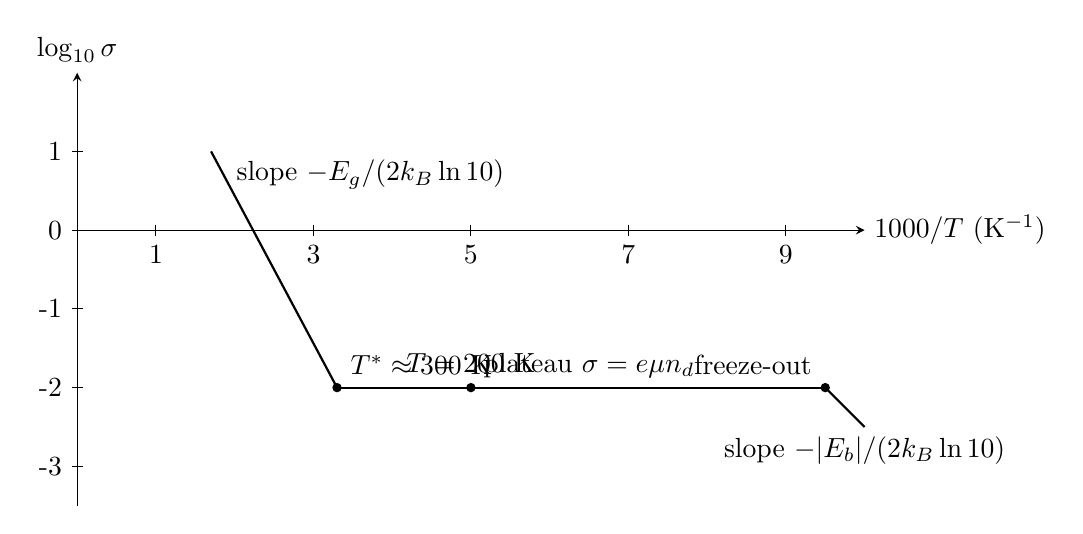
\begin{tikzpicture}[>=stealth, scale=1.0]
  % axes: x = 1000/T (K^-1), so x range covers 1000/600 ~ 1.7  to  1000/30 ~ 33.3
  \draw[->] (0,0) -- (10,0) node[right] {$1000/T\ (\si{K^{-1}})$};
  \draw[->] (0,-3.5) -- (0,2) node[above] {$\log_{10}\sigma$};
  % tick labels
  \foreach \x/\lab in {1/1, 3/3, 5/5, 7/7, 9/9}
    \draw (\x,0.07) -- (\x,-0.07) node[below] {\lab};
  \foreach \y/\lab in {-3/-3, -2/-2, -1/-1, 0/0, 1/1}
    \draw (0.07,\y) -- (-0.07,\y) node[left] {\lab};
  % intrinsic regime: steep negative slope from (1.7, +1) toward (3.3, -2)
  \draw[thick] (1.7,1.0) -- (3.3,-2.0);
  % extrinsic plateau from 1000/300 ~ 3.3 to 1000/73 ~ 13.7 ... but bounding box stops at 9.5
  \draw[thick] (3.3,-2.0) -- (9.5,-2.0);
  % freeze-out beyond x ~ 13.7 (offscreen); show small downward kink near right edge
  \draw[thick] (9.5,-2.0) -- (10,-2.5);
  % markers
  \node[circle,fill,inner sep=1.2pt,label=above right:{$T^*\approx 300$ K}] at (3.3,-2.0) {};
  \node[circle,fill,inner sep=1.2pt,label=above:{$T=200$ K}] at (5.0,-2.0) {};
  \node[circle,fill,inner sep=1.2pt,label=above left:{freeze-out}] at (9.5,-2.0) {};
  % slope labels
  \node[above right] at (1.9,0.4) {slope $-E_g/(2k_B\ln 10)$};
  \node[above] at (6.5,-2.0) {plateau $\sigma=e\mu n_d$};
  \node[below] at (10,-2.5) {slope $-|E_b|/(2k_B\ln 10)$};
\end{tikzpicture}
\end{center}

\boxed{\;\text{Steep intrinsic slope, flat extrinsic plateau at $\sigma=\SI{e-2}{\Omega^{-1}}$, freeze-out steep again at low $T$.}\;}

%======================================================================
\section*{Question 4 --- Magnetism of helium}

\subsection*{(a) Definitions}

\textbf{Paramagnet:} substance with positive magnetic susceptibility $\chi>0$; magnetisation aligns with applied field, vanishes when field is removed (e.g. unpaired spins).

\textbf{Diamagnet:} substance with negative susceptibility $\chi<0$; induced moment opposes applied field (universal Larmor response of closed shells).

\textbf{Ferromagnet:} substance with spontaneous magnetisation below a Curie temperature $T_c$, due to cooperative alignment of moments; $\chi$ diverges at $T_c$.

\subsection*{(b) Diamagnetic susceptibility of $^4$He}

\textbf{Problem.} \emph{What magnetic behaviour does $^4$He exhibit, and derive $\chi$ in terms of helium density, $\langle r^2\rangle$, fundamental constants.}

$^4$He is a closed-shell atom (1s$^2$, $S=L=J=0$) with no nuclear spin: purely \textbf{diamagnetic} (Larmor).

Minimal coupling $\bm p\to\bm p+e\bm A$ with $\bm A=\tfrac12\bm B\times\bm r$ gives, per electron:
\[
\Delta H = \frac{e^2}{8m_e}(\bm B\times\bm r)^2.
\]
Pick $\bm B=B\hat{\bm z}$:
\[
(\bm B\times\bm r)^2 = B^2(x^2+y^2).
\]
Substitute:
\[
\Delta H = \frac{e^2 B^2}{8m_e}(x^2+y^2).
\]
Spherical symmetry $\langle x^2\rangle=\langle y^2\rangle=\langle z^2\rangle=\langle r^2\rangle/3$:
\[
\langle x^2+y^2\rangle = \tfrac23\langle r^2\rangle.
\]
Multiply by 2 electrons per atom:
\[
\Delta E_{\text{atom}} = \frac{e^2 B^2}{8m_e}\cdot 2\cdot\tfrac23\langle r^2\rangle.
\]
Simplify:
\[
\Delta E_{\text{atom}} = \frac{e^2 B^2}{6 m_e}\langle r^2\rangle.
\]
Magnetisation per atom $m_{\text{atom}} = -\partial \Delta E_{\text{atom}}/\partial B$:
\[
m_{\text{atom}} = -\frac{e^2 B}{3m_e}\langle r^2\rangle.
\]
Multiply by number density $n$:
\[
M = -\frac{n e^2}{3m_e}\langle r^2\rangle\, B.
\]
Use $M=\chi H$ and $B=\mu_0 H$:
\[
\chi_{\text{dia}} = \frac{M}{H} = -\frac{n\mu_0 e^2}{3 m_e}\langle r^2\rangle.
\]
\[
\boxed{\;\chi_{\text{dia}} = -\frac{n\mu_0 e^2}{3 m_e}\langle r^2\rangle.\;}
\]

\subsection*{(c) Nuclear paramagnetic susceptibility of $^3$He}

\textbf{Problem.} \emph{Independent $^3$He nuclei, $\mu_{^3\text{He}}=-2.13\,\mu_N$, spin $1/2$. Find $\chi_{\text{nuc}}(T,n)$.}

Spin-$1/2$ nucleus in field $B$ has two levels $E_\pm = \mp |\mu| B$:
\[
Z_1 = e^{\beta|\mu| B} + e^{-\beta|\mu| B} = 2\cosh(\beta|\mu| B).
\]
Mean moment per atom $\langle m\rangle = \beta^{-1}\partial\ln Z_1/\partial B$:
\[
\langle m\rangle = |\mu|\tanh(\beta|\mu| B).
\]
Expand for $|\mu| B \ll k_B T$ (linear response):
\[
\langle m\rangle \approx \frac{|\mu|^2 B}{k_B T}.
\]
Multiply by density $n$:
\[
M = \frac{n|\mu|^2 B}{k_B T}.
\]
Apply $\chi = M/H = \mu_0 M/B$:
\[
\chi_{\text{nuc}} = \frac{n\mu_0 |\mu|^2}{k_B T}.
\]
Insert $|\mu| = 2.13\,\mu_N$:
\[
\boxed{\;\chi_{\text{nuc}}(T,n) = \frac{n\mu_0 (2.13\,\mu_N)^2}{k_B T}.\;}
\]

\subsection*{(d) Sign-change temperature}

\textbf{Problem.} \emph{Estimate $T$ at which total $\chi$ changes sign.}

Set total $\chi = \chi_{\text{dia}}+\chi_{\text{nuc}} = 0$:
\[
\frac{n\mu_0 (2.13\mu_N)^2}{k_B T^*} = \frac{n\mu_0 e^2}{3m_e}\langle r^2\rangle.
\]
Cancel $n\mu_0$:
\[
\frac{(2.13\mu_N)^2}{k_B T^*} = \frac{e^2 \langle r^2\rangle}{3m_e}.
\]
Solve for $T^*$:
\[
T^* = \frac{3 m_e (2.13\mu_N)^2}{k_B e^2 \langle r^2\rangle}.
\]
Estimate $\langle r^2\rangle\sim a_0^2$ with $a_0=\SI{0.529e-10}{m}$:
\[
\langle r^2\rangle \approx \SI{2.80e-21}{m^2}.
\]
Compute $(2.13\mu_N)^2$ with $\mu_N=\SI{5.05e-27}{J\,T^{-1}}$:
\[
2.13\mu_N = 1.076\times 10^{-26}\,\si{J\,T^{-1}}.
\]
Square:
\[
(2.13\mu_N)^2 = \SI{1.158e-52}{J^2\,T^{-2}}.
\]
Numerator:
\[
3 m_e (2.13\mu_N)^2 = 3\times 9.11\times 10^{-31}\times 1.158\times 10^{-52}.
\]
Evaluate:
\[
3 m_e (2.13\mu_N)^2 = \SI{3.165e-82}{kg\,J^2\,T^{-2}}.
\]
Denominator factors:
\[
e^2 = (1.602\times 10^{-19})^2 = \SI{2.566e-38}{C^2}.
\]
Combine:
\[
k_B e^2 \langle r^2\rangle = 1.381\times 10^{-23}\times 2.566\times 10^{-38}\times 2.80\times 10^{-21}.
\]
Evaluate:
\[
k_B e^2 \langle r^2\rangle = \SI{9.92e-82}{J\,C^2\,m^2}.
\]
Form ratio (using $1\,\si{J/T^2} = 1\,\si{C^2\,m^2/kg}$, so $kg \cdot J^2/T^2 = J\cdot C^2 m^2$, units of K from division by $k_B$):
\[
T^* \approx \frac{3.165\times 10^{-82}}{9.92\times 10^{-82}}\,\si{K}.
\]
Evaluate:
\[
T^* \approx \SI{0.32}{K}.
\]
\[
\boxed{\;T^* \sim \SI{0.3}{K}\ \text{(of order 100\,mK--1\,K).}\;}
\]

\subsection*{(e) Mean-field $T_c$ for bcc $^3$He}

\textbf{Problem.} \emph{Bcc $^3$He, $J_{nn}/k_B=\SI{1}{mK}$, $J_{nnn}/k_B=-\SI{0.5}{mK}$, spin $1/2$. Find $T_c$.}

Bcc lattice: $z_1=8$ nearest neighbours at coupling $J_1$, $z_2=6$ next-nearest at $J_2$. Effective sum:
\[
J_{\text{eff}} \equiv \sum_j J_{ij} = z_1 J_1 + z_2 J_2.
\]
Insert numbers:
\[
J_{\text{eff}}/k_B = 8(1) + 6(-0.5)\,\si{mK}.
\]
Simplify:
\[
J_{\text{eff}}/k_B = (8 - 3)\,\si{mK} = \SI{5}{mK}.
\]
Mean-field decoupling $\bm S_i\cdot\bm S_j\to\bm S_i\cdot\langle\bm S_j\rangle + \langle\bm S_i\rangle\cdot\bm S_j - \langle\bm S_i\rangle\cdot\langle\bm S_j\rangle$ on $H=-\tfrac12\sum_{i,j}J_{ij}\bm S_i\cdot\bm S_j$ gives effective single-site Hamiltonian:
\[
H_i^{\text{MF}} = -\bm S_i\cdot\bm h_{\text{eff}},\qquad \bm h_{\text{eff}} = \sum_j J_{ij}\langle\bm S_j\rangle = J_{\text{eff}}\langle\bm S\rangle.
\]
High-$T$ Brillouin self-consistency for spin $S$:
\[
\langle S\rangle = \frac{S(S+1)}{3 k_B T}\, h_{\text{eff}} = \frac{S(S+1)}{3 k_B T}\, J_{\text{eff}}\langle S\rangle.
\]
Non-trivial solution requires coefficient unity at $T_c$:
\[
k_B T_c = \frac{S(S+1)}{3}\, J_{\text{eff}}.
\]
Insert $S=1/2$, so $S(S+1)=3/4$:
\[
k_B T_c = \frac{1}{3}\cdot\frac{3}{4}\, J_{\text{eff}} = \tfrac{1}{4}\, J_{\text{eff}}.
\]
Evaluate:
\[
T_c = \tfrac{1}{4}\times \SI{5}{mK} = \SI{1.25}{mK}.
\]
\[
\boxed{\;T_c \approx \SI{1.25}{mK}.\;}
\]

\end{document}
